
%(BEGIN_QUESTION)
% Copyright 2006, Tony R. Kuphaldt, released under the Creative Commons Attribution License (v 1.0)
% This means you may do almost anything with this work of mine, so long as you give me proper credit

Both Bernoulli's and Torricelli's equations provide a mathematical relationship between pressure and flow rate, which means we should be able to measure pressure and thereby infer flow:

\vskip 10pt

{\bf Differential pressure resulting from pressure drop at venturi throat}:

$$\includegraphics[width=15.5cm]{i00453x01.eps}$$

\vskip 10pt

{\bf Hydrostatic pressure resulting from liquid column height}:

$$\includegraphics[width=15.5cm]{i00453x02.eps}$$

\vskip 10pt

One problem, though, is that the mathematical relationship in either of these scenarios is {\it not} linear.  Based on Bernoulli's and/or Torricelli's equations, what type of relationship is this?  What would we have to do to the pressure transmitter's signal to obtain a linear representation of flow?

\underbar{file i00453}
%(END_QUESTION)





%(BEGIN_ANSWER)

The relationship between pressure and flow is quadratic.

%(END_ANSWER)





%(BEGIN_NOTES)

$$P \propto Q^2$$

$$Q \propto \sqrt{P}$$

\noindent
Where,

$P$ = Pressure

$Q$ = Flow rate

\vskip 10pt

%INDEX% Physics, dynamic fluids: relationship between turbulent flow and pressure

%(END_NOTES)


